\section{Discussions} \label{s:discussions}
Throughout the extensive experiments conducted, we can notice that feature ranking based FVC techniques along with VC and CFC as the ensemble  technique have performed more accurately. In what follows we discuss these results from different angles and perspectives. 

\subsection{Feature ranking vs. w/o feature ranking}
From Figure \ref{F:MIMIC2_AdultK1F_Table} $-$ \ref{F:MIMIC3_Senior24hrs_Table}, the importance of feature ranking across different combinations of techniques and datasets is already evident. Figure \ref{F:Rank_Comparison_On_MIMICII_MIMICIII} here highlights this information in a more focused and systematic manner as follows.
%For each dataset this comparison is prepared. Figure \ref{F:MIMIC3_Senior24hrs_Table}, \ref{F:MIMIC2_AdultK1F_Table}, \ref{F:MIMIC2_AdultK1V_Table}, \ref{F:MIMIC2_SeniorK1F_Table}, \ref{F:MIMIC2_SeniorK1V_Table} and \ref{F:MIMIC3_Adult24hrs_Table} related to this section contains two information. One is the comparison of the proposed technique with w/o feature ranking approaches. Another one shows how much improvement achieved using proposed technique along with which techniques perform well. For these results, the highest $F_{wa}$ scores are presented to compare.  
The top left panel of Figure \ref{F:Rank_Comparison_On_MIMICII_MIMICIII} clearly reveals that for the MIMIC II Adult Binary (F) dataset when ranking based approaches are used with any FVC technique, the results are superior. It also hints that larger subsets of ranked features perform better. This may be attributed to the fact that among the features with positive (ranking) scores, there are not much difference with respect to importance (which is also evident from their very close importance scores). SVM and RF standout as the main performers as classifiers for doing better. 

\begin{figure}[h] 
	\centering 
	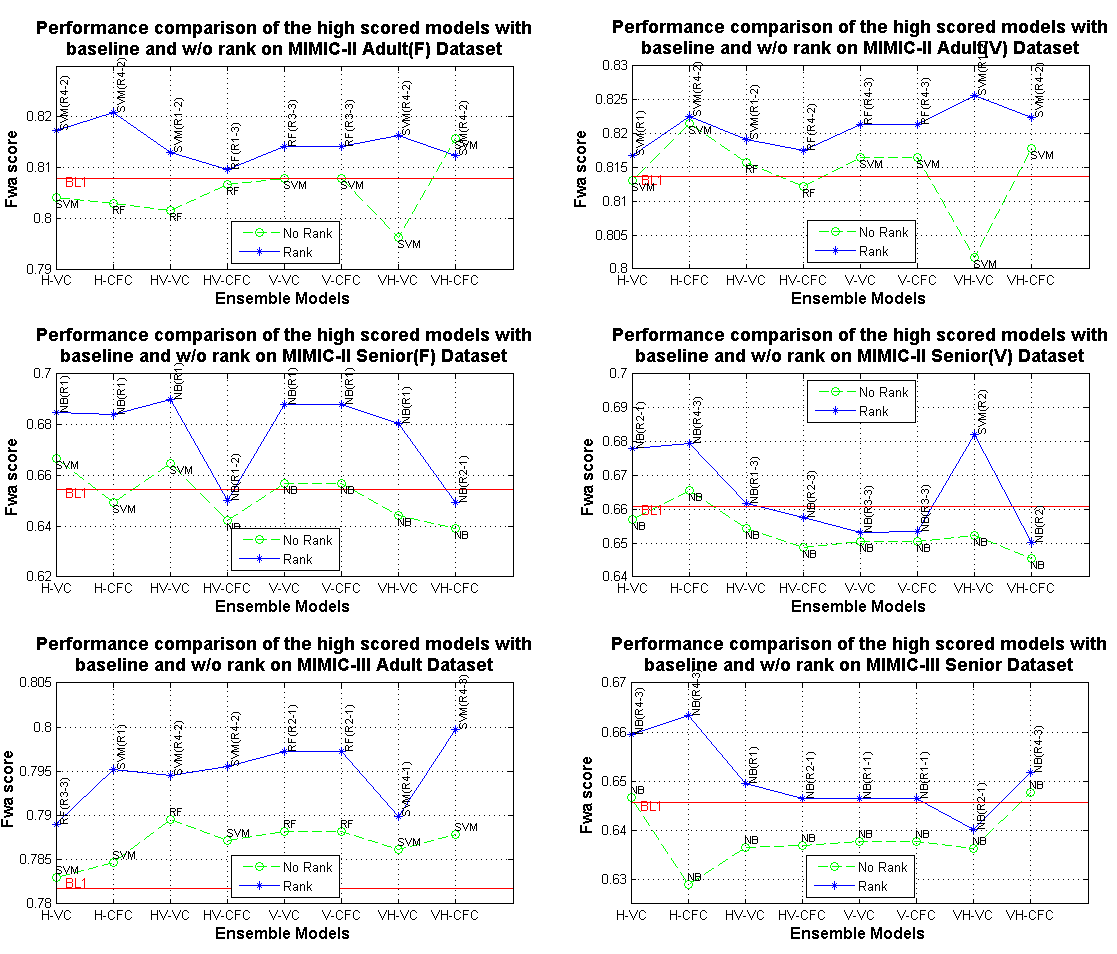
\includegraphics[scale=0.5]{fig/rank-comparison-on-all-datasets.png}
	\caption{Comparison of Feature ranking vs. w/o feature ranking based models in terms of $F_{wa}$ score on MIMIC-II and MIMIC-III datasets}
	\label{F:Rank_Comparison_On_MIMICII_MIMICIII}
\end{figure} 

The top right panel of Figure \ref{F:Rank_Comparison_On_MIMICII_MIMICIII} shows the results on MIMIC-II Adult Numeric (V) dataset. Here as well it is clearly evident that when ranking based approaches are used with any of the FVC techniques, then better results are achieved. Here SVM and RF are the star classifiers. 

The middle left panel of Figure \ref{F:Rank_Comparison_On_MIMICII_MIMICIII} demonstrates the results on MIMIC-II Senior Binary (F) dataset. It also indicates that when ranking based approaches are used with any of the FVC techniques, better results are achieved. Here the improvement is quite remarkable, i.e., 3.5\% improvement over BL1. Here NB is undoubtedly the best performer.

The middle right panel of Figure \ref{F:Rank_Comparison_On_MIMICII_MIMICIII} considers the MIMIC-II Senior Numeric (V) dataset. Here as well we notice the same situation with respect to feature ranking and the improvement is also mentionable, i.e., more than 2\%, over BL1. While NB here stands out with a robust performance overall, the best score is achieved by SVM. 

The bottom left panel of Figure \ref{F:Rank_Comparison_On_MIMICII_MIMICIII} focuses on MIMIC-III Adult dataset. Again the results are consistently in favour of feature ranking. Here NB is the star classifier. Finally, the bottom right panel of Figure \ref{F:Rank_Comparison_On_MIMICII_MIMICIII} focuses on MIMIC-III Senior dataset and the superiority of the combination with feature ranking is clearly evident here as well. For this dataset, NB is again the best performer. Interestingly, NB has performed consistently well for the Senior datasets of MIMIC-II and MIMIC-II, except for the Senior Numeric (V) dataset of MIMIC-II. 

To further check the direct contribution of the feature ranking and selection we have conducted some experiments without feature grouping. The results were better than BL1 in all datasets indicating that feature ranking directly contributes to the robustness of our approach.    

Apart from contributing through ranking and selection of features, feature ranking methodology is believed to have also helped us indirectly as follows. Many records of these datasets contain missing values. These missing values are replaced by the classifiers when the classifiers are trained. These replaced values may not be the true representation. When feature ranking based approach is used, some of these features are removed through the feature selection process thereby helping the classifier by removing `confusing' instances. \textcolor{blue}{For example, Protein S (Functional), Protein C (Functional), Reticulocyte Count (manual or absolute), Quantitative G6PD blood tests are found as low ranked features for Adult group in MIMIC-II and MIMIC-III datasets. Upon examination it has been found that in around 99\% cases the values of Quantitative G6PD, Protein C (Functional), and Protein S (Functional) are missing for Adult group in MIMIC-II datasets and in fact 100\% values of Reticulocyte Count blood test are missing for Adult group in MIMIC-III dataset. Similar situation is also observed for some other attributes/features as well (e.g., HLA-DR (Human Leukocyte Antigen – DR isotype), Heinz Body Prep, Howell-Jolly Bodies, and H/O Smear blood tests are found as low ranked features for Senior group in MIMIC-II datasets as these are missing in around 99\% cases.). Thus the feature ranking \& selection step acted as a filter excluding these 'damaging' features thereby improving the classifier performance.}

\subsection{Feature ranking implications}
In an effort to analyze and understand the implications of feature ranking we have identified the top ten features (based on ranking) of each dataset which are listed in the supplementary document. For every dataset some features, such as, Red blood cell Distribution Width (RDW), Creatinine, Bilirubin, and Urea Nitrogen are found within the top ranked features. From medical perspective these features are very important for a patient and specially when he is at ICU. For example, RDW mainly confirms the presence of anemia. It is also used to evaluate critical conditions, like, cancer, heart disease, liver disorder etc. \textcolor{blue}{In a recent study \cite{Fernandez2018} it has been seen that high RDW is a marker of severity at ICU discharge in the context of in-hospital mortality.} Similarly, high creatinine level indicates kidney disease or a dysfunctional kidney. Thus ranking algorithms have been able to correctly capture these as some of the highly important features among others. Thus, not surprisingly, feature ranking based models have performed better as compared to the baselines.   

We have also performed a statistical correlation analysis on some top ranked features and the patient status (alive/dead). These results are reported in the supplementary file. For each important feature, we estimated the degree of association between that feature and the patient status by fitting a simple linear regression model. Then we assessed the statistical significance of each inferred association using hypothesis testing. We applied the t-test assuming that there is no association which is known as the null hypothesis. The resultant p-value showed us the probability of obtaining a result equal to or ``more extreme" than what was actually observed, when the null hypothesis is true. For all the associations, we obtained p-value 0.0 (rounded to 5 decimal point). So with 99\% confidence we can state these associations to be significant. These results further strengthen our hypothesis that feature ranking and selection was fruitful.        

\subsection{VC vs. CFC}
VC and CFC techniques are used as the ensemble approach to find the right classifier from the ensembles for test instance to do the prediction. The contribution of these techniques depends on the structure of the records of ensemble clusters (through FVC technique) and the structure of the test instance. VC mainly focuses on the missing values present in the ensemble cluster and the test record whereas contrastingly, CFC checks for the common values between the two. Therefore, more missing values guides VC and less missing values aid CFC. 

The results shown in Figure \ref{F:Rank_Comparison_On_MIMICII_MIMICIII} indicate that CFC technique is better for MIMIC-III datasets as compared to VC technique during ensemble classification process. The available features and their values (including missing ones) seen in the datasets of MIMIC-II and MIMIC-III are primarily responsible for these outcomes. For MIMIC-III datasets as compared to MIMIC-II less missing values are found during the ensemble clustering process. Therefore, CFC is performing better for MIMIC-III datasets.             

%The structure of the instances and the availabilities of the feature values in these instances seen in the datasets of MIMIC-II and MIMIC-III are primarily responsible for these outcomes. For MIMIC-III datasets, a test instance gets the closest classifier in terms of CFC value during classification process mostly due to the feature values presentation. Therefore, CFC is performing better for these datasets.            

%\subsubsection{HV vs. H vs. VH vs. V}
%Feature vector compaction techniques depends on primarily vacuum counting between two instances. Therefore, these depend on how much missing values are present in the datasets. From data shown in Figures \ref{F:Rank_Comparison_On_MIMICII_MIMICIII} and results of each dataset of MIMIC-II and MIMIC-III, one thing has been observed that for MIMIC-II numeric datasets (e.g., Adult(V), Senior(V)) VH grouping doing better results. For other datasets these FVC techniques are varied.   
 
\subsection{Results comparing with baselines}
\textcolor{blue}{In the context of mortality or survival prediction of ICU patients, most of the studies \cite{Pirracchio2015, Calvert2016, Bhattacharya2017, Xie2017, Awad2017, Johnson2nd2017, Darabi2018, Davoodi2018, Sadeghi2018, Purushotham2018} found in literature mainly work with vital signs with lab tests to predict the mortality of ICU patients. Some of other works, such as \cite{Ghassemi2015, Marafino2015, Grnarova2016, ZhengpingChe2016}, primarily focus on clinical notes along with these variables. To the best of our knowledge, we found only two works \cite{mehedy-masud:2017:fvc, mehedy-masud:2018:frmwrk} that focus on only lab tests results. Therefore, we compare our results with these studies. Figure \ref{F:comparison_with_state_of_art}, Table \ref{t:Summary_of_results_with_all_baselines2}, and Table \ref{t:Summary_of_results_with_all_baselines} present our results comparing with these relevant studies and show the improved performances in all matrics.}  

\textcolor{blue}{Johnson \textit{et al.} conducted a study to reproduce the cohorts used in some studies in the context of performance comparison of the mortality prediction models for the ICU patients using MIMIC datasets \cite{Johnson2nd2017}. They stated that the accurate reproduction of the studies found in the literature can't be guaranteed in this context but their results may be compared by following consistent model design and methodology. In our study, we have followed this principal and present our results comparing with all baselines from the relevant studies \cite{mehedy-masud:2017:fvc, mehedy-masud:2018:frmwrk}.}

\textcolor{blue}{Most of the studies found in the literature either work on MIMIC-II dataset or MIMIC-III dataset as reported in the comparison of benchmark works in a recent study \cite{Purushotham2018}. Purushotham \textit{et al.} performed this study \cite{Purushotham2018} to present benchmark results in the context of some clinical prediction tasks (such as mortality prediction, LoS prediction, and ICD-9 code group prediction). They conducted experiments on MIMIC-III database and formed three sets of features as follows. Feature set A contains 17 features (pre-processed) used in the calculation of the SAPS-II score. Feature set B contains 20 features corresponding to 17 pre-processed features used in Feature set A. Here raw values of the features are used instead of pre-processed ones. Feature set C contains 136 features with raw values. In this set, 20 features of feature set B are available. In these feature sets, vital signs are primary features. On the other hand, our study mainly focus on lab test records for MIMIC-II and MIMIC-III datasets. We have conducted our experiments on a large set of lab tests, namely, 655 lab tests from MIMIC-II datasets and 570 lab tests from MIMIC-III datasets.}  
 
\subsection{About feature sets used here}
\textcolor{blue}{As has been discussed while reviewing the literature we could not find any research work that only considers lab test results for mortality prediction. Here we bring about that discussion in a more focused manner. The works of Calvert \textit{et al.} \cite{Calvert2016}, Johnson \textit{et al.} \cite{Johnson2nd2017}, and Purushotham \textit{et al.} \cite{Purushotham2018} exploited some lab test results (along with other features) in their models. All those lab test results have been included in our feature set. Caicedo-Torres and Gutierrez also used few lab tests in their study \cite{Torres2019}. All these lab tests are included in our feature sets.} 
